\documentclass[10pt]{article}

\usepackage[margin=1in]{geometry}
\usepackage{amsmath,amssymb}
\usepackage{graphicx}
\usepackage{hyperref}

\title{Best-of-N Inference Can Exploit Proxy Scores in Flow-Matching World Models}
\author{Anonymous Authors}
\date{}

\begin{document}
\maketitle

\begin{abstract}
Flow-matching and rectified-flow models offer fast conditional generation of continuous trajectories, making them attractive as world models for planning. A tempting inference strategy is to sample many candidate futures and select the one with the largest learned value score. We study this Best-of-N procedure in a controlled synthetic setting. A conditional rectified-flow trajectory generator is trained on two-mode point-mass trajectories around an obstacle, while a misspecified proxy value model reranks generated futures. We find that increasing the candidate budget can improve proxy score while selecting trajectories with larger true-vs-predicted gaps and greater feature-space distance from the training manifold. A simple uncertainty penalty reduces this exploitation in the synthetic task. The result is best read as a diagnostic pilot: the parent phenomenon is reward-model overoptimization, and the contribution is a concrete measurement harness for flow-generated world-model trajectories.
\end{abstract}

\section{Introduction}

World models support planning by predicting futures under candidate actions. Flow-matching and rectified-flow models are appealing for this role because they learn vector fields that transport simple noise into structured samples with few ODE steps. Once such a model can generate whole trajectories, a natural planner is Best-of-N inference: sample $N$ futures, score each with a value model, and execute or study the highest-scoring candidate.

This paper asks whether that interface is safe under proxy error. Prior work on reward-model overoptimization already shows that Best-of-N can Goodhart an imperfect reward model. The narrower question here is what that looks like for continuous trajectories sampled from a conditional rectified-flow world model. We focus on diagnostics: selection bias, selected trajectory diversity, feature-space out-of-distribution distance, and true-vs-predicted return gap.

\section{Setup}

The synthetic environment is a two-dimensional point mass. Each context specifies a goal height, obstacle radius, and lateral wind coefficient. Expert trajectories move from $(0,0)$ to $(1,g_y)$ using one of two modes around the obstacle. The generator is trained as a rectified flow: for data trajectory $x_1$, Gaussian base sample $x_0$, and interpolation time $t$, the model predicts
\[
v_\theta((1-t)x_0 + t x_1, t, c) \approx x_1 - x_0.
\]
At inference, Euler integration maps Gaussian noise to candidate trajectories conditioned on context $c$.

The proxy value model is a ridge-regression scorer trained on expert trajectories. It deliberately omits direct obstacle-collision and monotonicity features, so it is accurate near the expert manifold but vulnerable when reranking searches unusual generated samples. The true return penalizes endpoint error, collision depth, path roughness, path length, and backward motion.

\section{Best-of-N And Repair}

For each context, candidates $\{x_i\}_{i=1}^N$ are sampled from the flow model and scored by a proxy $\hat R(x_i,c)$. Naive Best-of-N selects
\[
i^\star = \arg\max_i \hat R(x_i,c).
\]
The repair baseline estimates feature-space uncertainty $u(x,c)$ from training trajectories and selects
\[
i^\star_\lambda = \arg\max_i \hat R(x_i,c) - \lambda u(x_i,c).
\]
This is not proposed as a new general algorithm. It is a robust reranking sanity check.

\paragraph{Bound.}
Assume $|R(x_i,c)-\hat R(x_i,c)| \le \beta u(x_i,c)$ for all candidates. Let $j$ be any candidate and let $i^\star_\beta$ maximize $\hat R(x_i,c)-\beta u(x_i,c)$. Then
\[
R(x_{i^\star_\beta},c) \ge R(x_j,c) - 2\beta u(x_j,c).
\]
The proof follows by lower-bounding the selected candidate by its penalized proxy objective and upper-bounding the comparison candidate's proxy by its true return plus uncertainty. The proposition is only a calibration lens; the experiment does not prove that the bound holds in general.

\section{Experiment}

We run a smoke-scale experiment with fixed random seed. The diagnostics in Figure~\ref{fig:diagnostics} compare random first-candidate selection, proxy-only Best-of-N, and uncertainty-penalized Best-of-N as $N$ increases.

\begin{figure}[h]
\centering
\begin{minipage}{0.48\linewidth}
\centering
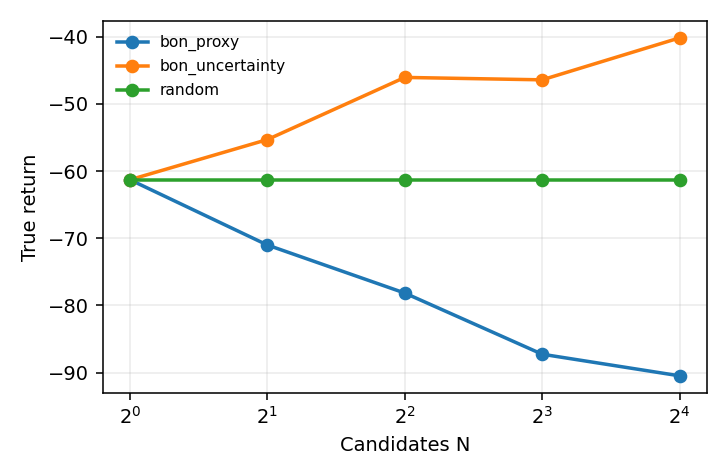
\includegraphics[width=\linewidth]{figures/return_vs_n.png}
\end{minipage}
\begin{minipage}{0.48\linewidth}
\centering
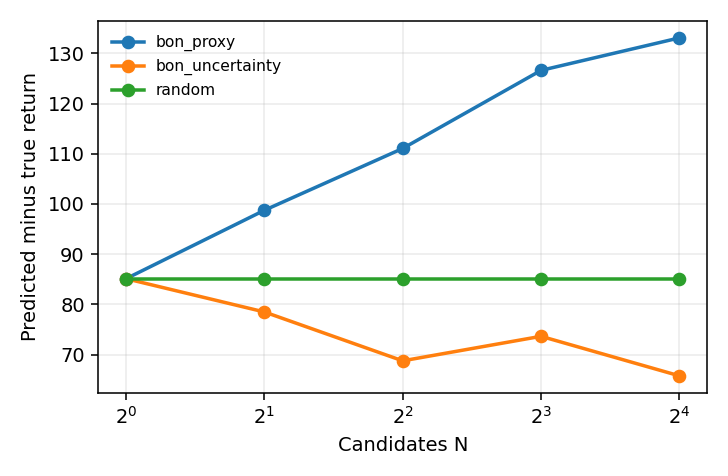
\includegraphics[width=\linewidth]{figures/gap_vs_n.png}
\end{minipage}

\vspace{0.4em}
\begin{minipage}{0.48\linewidth}
\centering
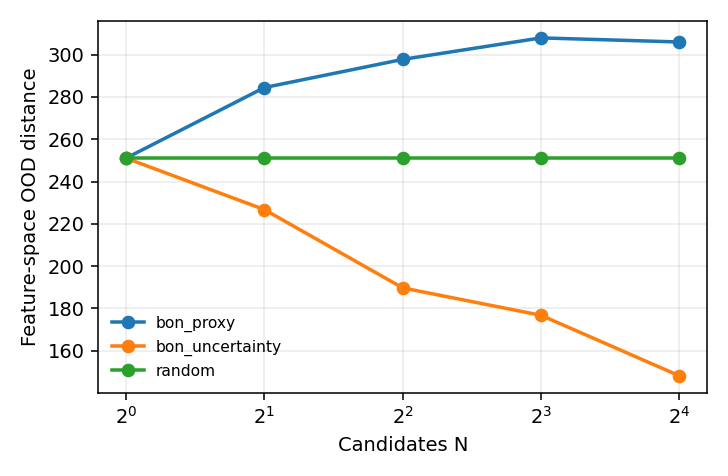
\includegraphics[width=\linewidth]{figures/ood_vs_n.png}
\end{minipage}
\begin{minipage}{0.48\linewidth}
\centering
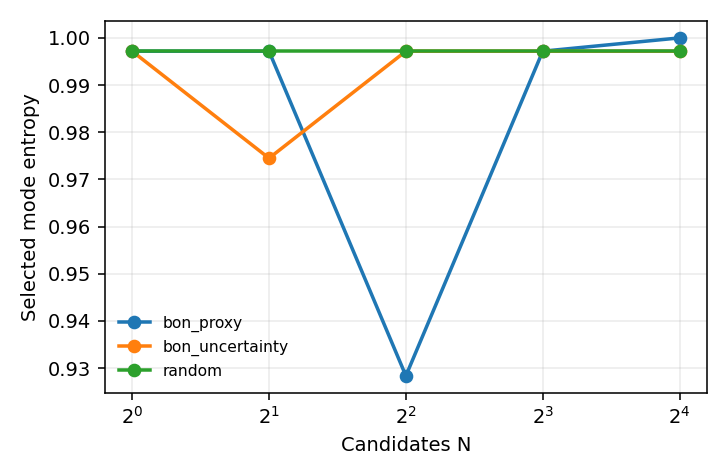
\includegraphics[width=\linewidth]{figures/diversity_vs_n.png}
\end{minipage}
\caption{Smoke diagnostics for Best-of-N reranking. Proxy-only selection tends to increase predicted return and selection bias, but can also increase true-vs-predicted gap and feature-space OOD distance. The uncertainty penalty is a small repair baseline, not a complete solution.}
\label{fig:diagnostics}
\end{figure}

\section{Related Work}

Flow Matching introduced simulation-free vector-field training for continuous normalizing flows, and Rectified Flow specialized this view around straight transports. Stochastic interpolants and probability-flow ODEs make clear that many sampling issues are shared across flow and diffusion families. World-model methods such as PlaNet, Dreamer, DreamerV3, EfficientZero, and TD-MPC2 provide stronger full-control baselines than the toy system here. Diffuser and Decision Diffuser are close neighbors because they cast decision making as generative trajectory modeling. Best-of-N reward-model overoptimization, especially the scaling-law analysis of Gao, Schulman, and Hilton, is the direct parent phenomenon. This work should therefore be read as a flow-trajectory diagnostic, not as a discovery of Goodhart effects.

\section{Discussion}

The evidence supports a modest conclusion: in a controlled rectified-flow trajectory generator, increasing the candidate budget can move selection toward proxy-exploiting samples. A feature-space uncertainty penalty reduces the effect in the smoke setting. The main value of the repo is the harness: it makes selection bias, diversity collapse, OOD distance, and true-vs-proxy gaps visible in one small experiment.

The next version should add a diffusion trajectory baseline, learned uncertainty, stronger value models, and standard offline-control tasks. Without those additions, the paper is a first-pass artifact rather than a complete ICLR-ready empirical result.

\begin{thebibliography}{9}

\bibitem{lipman2023}
Y. Lipman, R. T. Q. Chen, H. Ben-Hamu, M. Nickel, and M. Le.
Flow Matching for Generative Modeling.
ICLR, 2023.

\bibitem{liu2023}
X. Liu, C. Gong, and Q. Liu.
Flow Straight and Fast: Learning to Generate and Transfer Data with Rectified Flow.
ICLR, 2023.

\bibitem{gao2023}
L. Gao, J. Schulman, and J. Hilton.
Scaling Laws for Reward Model Overoptimization.
ICML, 2023.

\bibitem{janner2022}
M. Janner, Y. Du, J. Tenenbaum, and S. Levine.
Planning with Diffusion for Flexible Behavior Synthesis.
ICML, 2022.

\bibitem{hafner2023}
D. Hafner, J. Pasukonis, J. Ba, and T. Lillicrap.
Mastering Diverse Domains through World Models.
arXiv, 2023.

\end{thebibliography}

\end{document}
